\section{Implementierung (Joshua Hörmann)}
Dieses Kapitel beschäftigt sich mit der eigentlichen Implementierung des Artbots. Zu diesem Zweck wird zuerst auf die verwendeten Tools \& Libraries eingegangen, um dann die konkrete Umsetzung und den Zusammenhang zu erklären.
\subsection{Tools \& Libraries}
\paragraph{Rasa}
Die Grundlage des ArtBots bildet das Rasa Framework. Rasa ist ein Open-Source Framework, welches zur Entwicklung von Chatbots mithilfe von Machine Learning eingesetzt wird. Dabei ist Rasa in zwei Hauptteile aufgeteilt: Rasa NLU (Natural Language Understanding) und Rasa Core. Dabei kümmert sich Rasa NLU um alles, was Natural Language Processing (NLP) betrifft und extrahiert die wichtigen Aussagen. Daraufhin kümmert sich Rasa Core um das Dialog Management und die Erstellung der Antworten des Chatbots \cite{rasa_definition}. Dies ist nur eine sehr grobe Beschreibung von Rasa, deutlich detaillierter ist es unter \ref{sec:flow} bzw. \cite[S.9f]{seminar} beschrieben.
\paragraph{Chatbot Widget designed for Rasa Bots}\label{chatbot_widget}
Für das Frontend wurde 'Chatbot Widget designed for Rasa Bots' von Jitesh Gaikwad verwendet \cite{chatbot_widget}. Dies ist ein Open Source Frontend, welches mit Javascript programmiert ist und sich leicht in Webseiten einbinden lässt. Es kommuniziert mit Rasa über sogenannte REST Channels. REST steht für Representational State Transfer und ist ein geläufiges Konzept für APIs. Dabei stellt der Rasa-Bot eine URL bereit, an welche das Chatbot Widget Requests senden kann und basierend darauf schickt Rasa dann einen entsprechenden Response an das Chatbot Widget zurück. \cite{rest}
\paragraph{Chatito}\label{chatito}
Um das Erstellen von Trainings- und Testdaten zu vereinfachen wurde Chatito verwendet. Chatito ist ein Projekt von Rodrigo Pimentel, welches eine Online Entwicklungsumgebung auf Github bereitstellt. \cite{chatito_ide} In dieser Online IDE kann man mit wenigen Eingaben in einer leicht verständlichen Syntax Datensätze erstellen. Diese Datensätze werden als JSON-Files ausgegeben, können also nicht nur mit Rasa sondern auch mit anderen Frameworks verwendet werden. Mehr zu der Funktionsweise von Chatito kann unter \cite{chatito_spec} nachgelesen werden.
\subsection{Umsetzung}\label{umsetzung}

\begin{figure}[H]
	\centerline{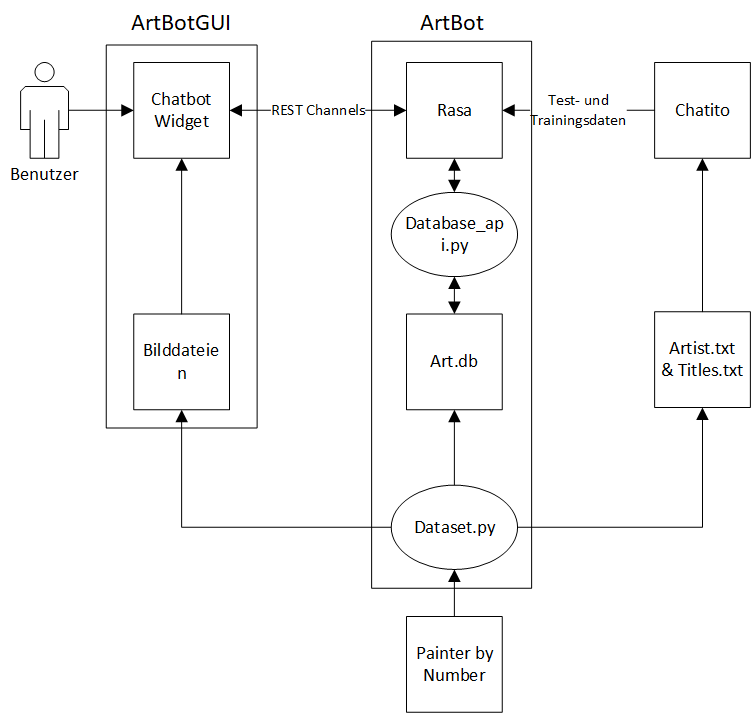
\includegraphics[width=0.8\linewidth]{figures/implementierung.png}}
	\caption{Der Aufbau und die Interaktion des ArtBots}
	\label{img:implemenatation}
\end{figure}

Die Abbildung \ref{img:implemenatation} gibt einen Überblick über den Aufbau und die Interaktionen innerhalb der entwickelten Anwendung. Ebenso kann man anhand der Abbildung die Struktur des Projekts sehen. Der Benutzer interagiert mit dem Chatbot Widget, welches zusammen mit den Bilddateien die ArtBotGUI bildet. Hierbei liegen die Bilddateien innerhalb von \textbackslash ArtBotGUI\textbackslash static\textbackslash art. In dem Ordner ArtBotGUI sind alle weiteren Dateien des Chatbot Widgets abgelegt. Diese GUI interagiert über REST Channels mit dem Rasa Chatbot, der mit der Datenbank Art.db, der Datenbank API Database\_api.py und dem Pythonscript Dataset.py zum Erstellen der Datenbasis den ArtBot bildet. All diese Dateien befinden sich in dem Ordner ArtBot, zusätzlich sind hier diverse Dateien von Rasa vorhanden, wie zum Beispiel die Testdaten in train\_test\_split oder die config.yml. Außerhalb des ArtBots und der GUI befindet sich der Datensatz, woraus mithilfe von Dataset.py die Datenbank und die Bilddateien extrahiert werden. Zusätzlich erzeugt dieses Pythonprogramm noch die zwei Textdateien Artist.txt und Titles.txt, welche zum Erstellen der Trainings- und Testdaten in Chatito benötigt werden. Die von Chatito erzeugten Datensets werden dann wiederum in Rasa innerhalb des ArtBots für das Training verwendet. 